\section{Android App}
This section presents the work done so fare in the smart phone application to monitor the charging status of the battery cells. The application is based on the android mobile operating system and it functions  as a graphical user interface for the hardware to display the charge of the battery. You can download the software following the same steps given in Sec.\ref{sec:userMan}

\vspace{0.3cm}%
\noindent\colorbox{myLavender!15}{\parbox{\textwidth}{\vspace{0.1cm}%
        The full code can be found at: \url{https://github.com/mnourgwad/imhotep}
        \vspace{0.1cm}}}

\begin{enumerate}
\item Copy the app \texttt{apk} file from the folder:\\
\url{imhotep/androidStuff/code/app/build/outputs/apk/debug/app-debug.apk}
\item to your phone and install it follow any of these tutorials:
    \begin{itemize}
        \item \url{https://www.techbout.com/install-apk-files-pc-android-3323}
        \item \url{https://www.wikihow.com/Install-APK-Files-from-a-PC-on-Android}
        \item \url{https://www.wikihow.tech/Install-APK-Files-on-Android}
    \end{itemize}
    \item It starts with prompting the user to enter the connection information for the Arduino.
    \begin{figure}[h]
        \centering
        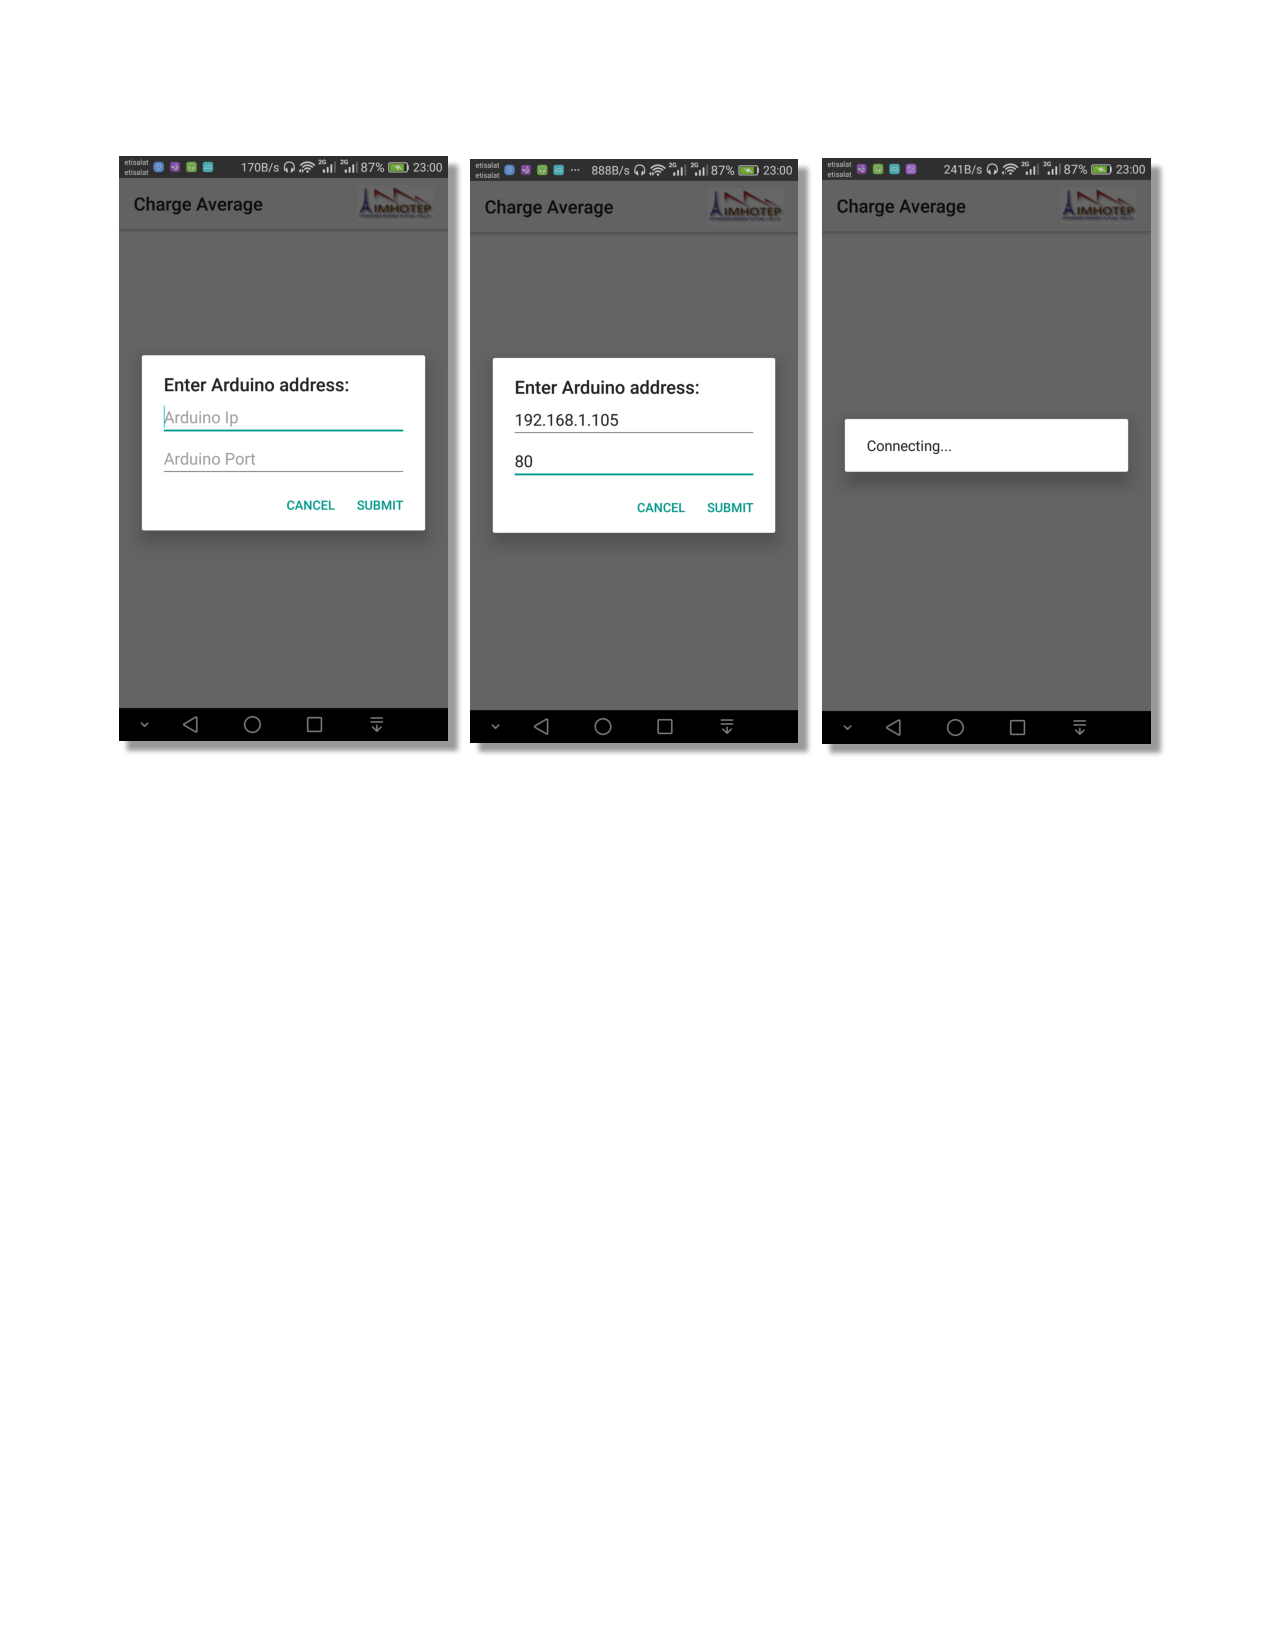
\includegraphics[width=0.8\textwidth,page=1]{figures/androidFigs}
        \caption{Connecting to the BMS hardware}
        \label{fig:appConfig}
    \end{figure}
    \item On submitting, the application tries to connect to the Arduino with timeout of 10 seconds.
    \item After establishing the connection, the application starts to query the Arduino for some information such as (the number of batteries, the max reading, the conversion factor and the reading for each battery.
    \item The application then display the average reading for the batteries in the main view with the percentage of the charge.
    \begin{figure}[h]
        \centering
        \includegraphics[width=0.6\textwidth,page=2]{figures/androidFigs}
        \caption{App displaying the average charge of all batteries (left) and the detailed charge for each one (right).}
        \label{fig:appCharge}
    \end{figure}
    \item On touching the view, the application displays the charge for each battery alone.
    \item There is an options menu on the right side of the action bar for the user to change the config data such as the max charge for the batteries and to try to reconnect or change the connection information to the Arduino.
    \begin{figure}[H]
        \centering
        \includegraphics[width=0.6\textwidth,page=3]{figures/androidFigs}
        \caption{App settings.}
        \label{fig:appSettings}
    \end{figure}
\end{enumerate}




\subsection{Android App Flowchart}
The flowchart for the main components of the android app is given in Fig.\ref{fig:Flowchart}.
\begin{figure}[h]
    \centering
    \includegraphics[width=\textwidth,page=4]{figures/androidFigs}
    \caption{Flowchart for the main components of the app.}
    \label{fig:Flowchart}
\end{figure}


\subsection{To Edit the Code}
\begin{enumerate}
    \item Open the code in Android Studio 3.0.1 or later.
    \item Download the SDK versions 21 and 26 as the min. and max. APIs for the application to build from \textbf{File} $>$ \textbf{Settings} $>$ \textbf{Appearance \& Behavior} $>$ \textbf{System Settings} $>$ \textbf{Android SDK }and mark the required APIs (check Fig.\ref{fig:SDKsetup}). \\
     \item Download the gradle version 4.1 to build the application.
        \begin{figure}[h]
            \centering
            \includegraphics[width=0.8\textwidth,page=5]{figures/androidFigs}
            \caption{Android Studio and SDK setup}
            \label{fig:SDKsetup}
        \end{figure}
    \begin{itemize}
        \item You can find these tools at:\\
        \url{https://developer.android.com/studio/index.html}\\
        \url{https://gradle.org}
    \end{itemize}
\end{enumerate}

\subsection{Applying the Test}
     To run the apk, you need a device with Android OS version 5.0 (Lollipop) or later to version 8.0 (Oreo). On the Arduino side, we used Nodemcu board - It is an Arduino compatible board with ESP8266 \textbf{WiFi module} implemented on it.
\begin{figure}[H]
    \centering
    \includegraphics[width=0.4\textwidth,page=6]{figures/androidFigs}
    \caption{Flowchart for the applicatio}
    \label{fig:Flowchart}
\end{figure}
I have provided a demo test code for the Arduino side. You can find it at the folder:\\
\url{imhotep/androidStuff/arduino_demo/WiFiWebServer/WiFiWebServer.ino}

When running this demo test code on the Arduino board, the board starts with trying to connect to the network specified in the code and on a successful connection, it prints out its IP address so we can access it from the android app.